\newpage
\newpage
\section{Flexible tube}
This benchmark details fluids in flexible cylindrical tubes \cite{Greenshields2005}, which is relevant to practical problems as pressure surge in pipelines and blood flow in arteries. Specifically this deals with wave propagation due to pressure drop. Pressure will be added to one side of the cylinder producing a wave in which theoretical wave and flow speed can be calculated and compared to numerical findings.

\subsection{Problem definition}
\begin{center} 
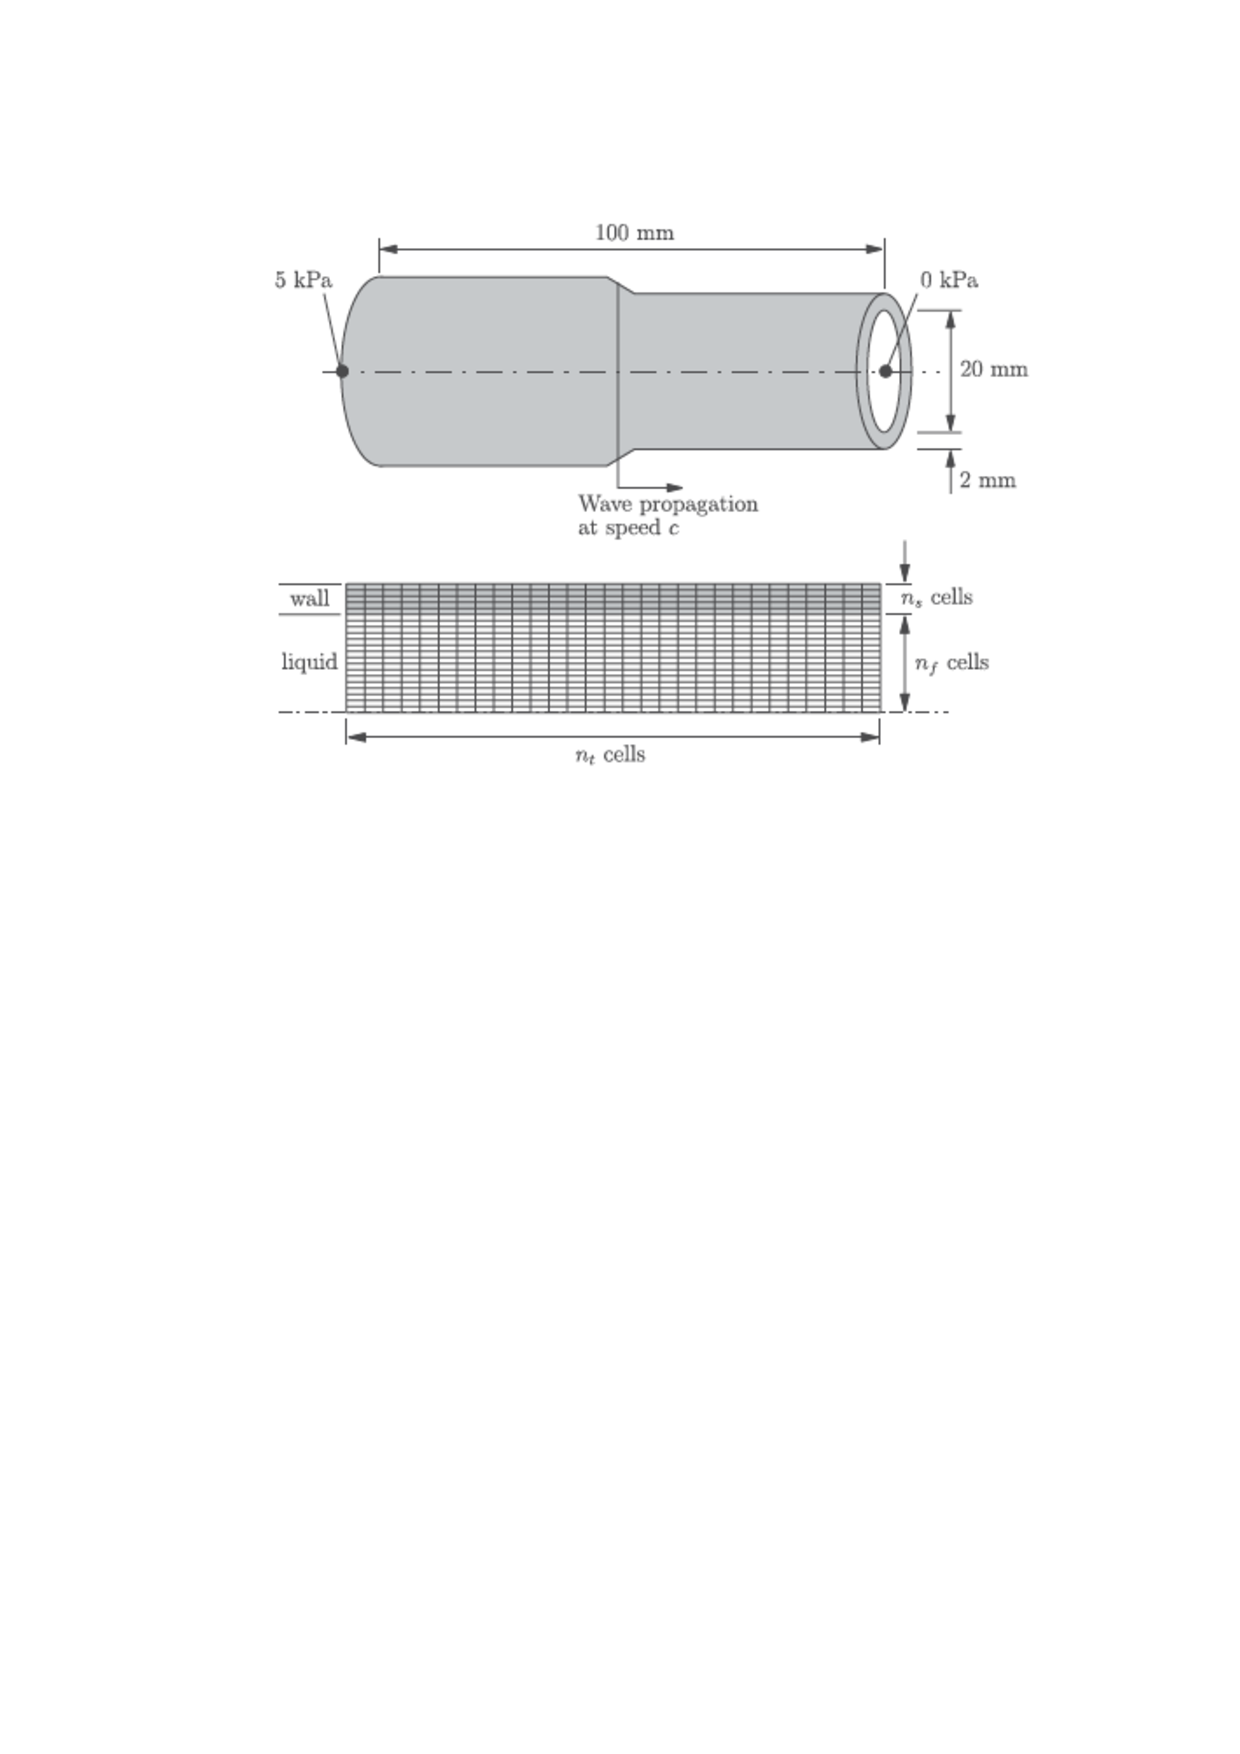
\includegraphics[scale=0.6,trim={0 15cm 0 10},clip]{./Verification_Validation/Flexible_tube/Pictures/definition.pdf}
\end{center}

The properties and geometry were selected for its representation of blood flow in a large artery. 

\subsection{Boundary conditions}


\subsection{Quanities for comparison}

\subsection{Results}
\begin{table}[h!]
\centering
\caption{My caption}
\label{my-label}
\begin{tabular}{|l|l|l|l|l|l|l|l|l|l|l|}
\hline
l {[}mm{]} & D {[}mm{]} & t {[}mm{]} & E {[}MPa{]} & $K_s [kPa] $ & $K_f [GPa]$ & $\nu_s $ & $\rho_s [\frac{kg}{m^3}]$ & $ \mu_s [kPa]  $ & $\rho_f []$ & $\mu_f [\frac{Ns}{m^2}]$ \\ \hline
100 & 20 & 2 & 1 & 833 & 2.2 & 0.3 & 1000 & 385 & 1000 & 0.0004 \\ \hline
\end{tabular}
\end{table}